\section{Experiments and Results}

In this section we will go in detail over the experiments we have conducted to evaluate the performance of our model, implementation choices, problems we encountered and how we solved them. Given the limited training capacity of the available computing resources, most architectural decisions were made with a trade-off between model complexity and training time, which may have resulted in suboptimal performance and the reason why the model is not able to transfer the style.

\subsection{Training environment}

The training was conducted on a single NVIDIA GeForce RTX 3060 Ti GPU with 8GB of VRAM. We were bound by this limitation in choosing the model architecture and the hyperparameters, which may have directly resulted in the suboptimal performance of the model and lack of convergence, even if we worked on such a reduced dataset of 128x128 grayscale spectrograms.

\vspace{1em}

\noindent We developed two training scripts, one for the pre-training phase and one for the main training of the LDM. The trained weights of the autoencoder are then loaded into the LDM and frozen.

\begin{lstlisting}[language=bash, basicstyle=\tiny]
# Pre-training the autoencoder
python models/train.py --model autoencoder

# Training the latent diffusion model
python models/train.py --model ldm
\end{lstlisting}

\noindent The hyperparameter configuration is available in the \texttt{config.py} file.


\subsection{Spectogram resolution}

We experimented with different spectogram resolutions, by manually inspecting the reconstructed audio. We decided on using 128 frequency ranges for the spectrograms, as it provided a good balance between quality and training time and limiting the temporal resolution to 3 seconds.

\subsection{Pre-training the compression model}

The compression model (encoder and decoder) are jointly pre-trained on the training set for 100 epochs using a learning rate of 0.5e-4 with an AdamW optimizer and ReduceLROnPlateau scheduler. The learning rate is reduced by a factor of 0.5 when the validation loss plateaus for 10 epochs, with a minimum learning rate of 1e-6. This adaptive learning rate strategy helps prevent overfitting and ensures stable convergence of the compression model training.

The pre-training phase focuses solely on reconstruction quality, optimizing the encoder-decoder architecture to effectively compress and reconstruct the input spectrograms while preserving essential musical features. This step is crucial as it establishes a strong foundation for the latent space that will later be used by the diffusion model for style transfer. We decide to regularize our latent space using a KL divergence loss, which helps to ensure that the latent space is normally distributed. Both the encoder and decoder are fully convolutional, allowing for dynamic input sizes.

We originally experimented with a latent space dimension of [32,8,8], which we found out to be too limiting in terms of the expressiveness of the latent space. We increased the spatial resolution of the latent space to [32,16,16], which allowed the model to learn a more complex latent space and improve the quality of the style transfer.

\begin{figure}[h]
    \centering
    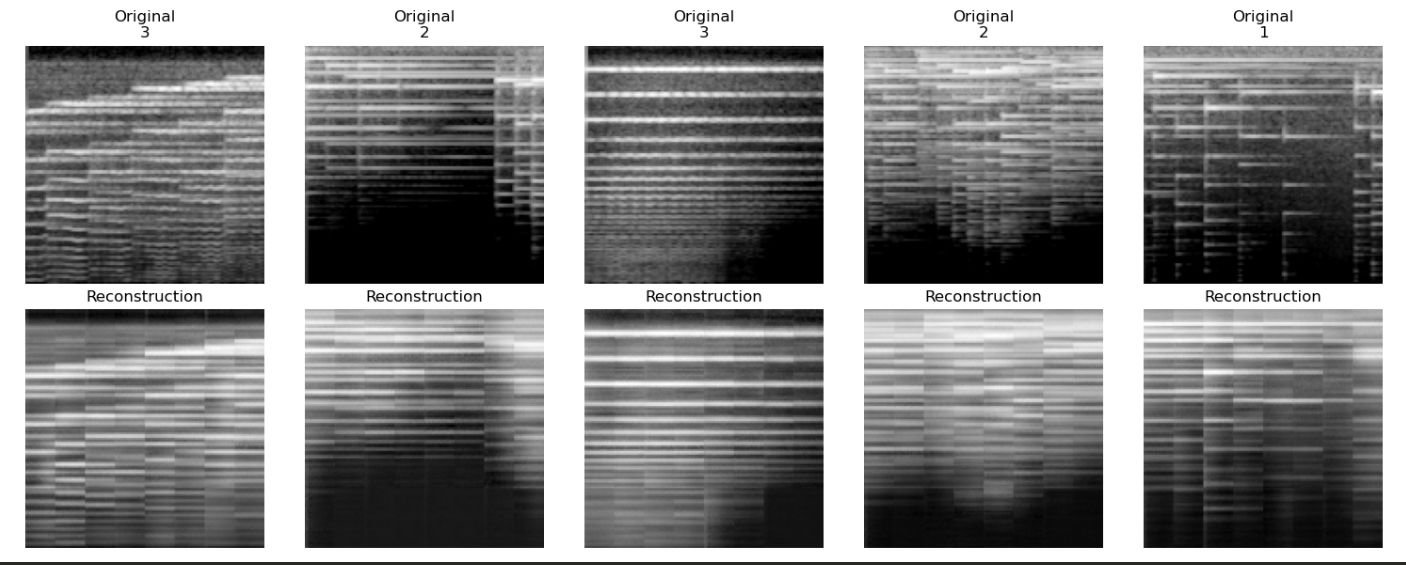
\includegraphics[width=\textwidth]{figures/reconstruction.jpeg}
    \caption{Reconstruction results from the pre-trained autoencoder. The first row shows the input spectrograms, while the second row shows the reconstructed spectrograms. }
    \label{fig:reconstruction}
\end{figure}

\noindent At this point we are able to reconstruct the input spectrograms with a high degree of accuracy, as shown in Figure \ref{fig:reconstruction}. We now freeze the weights of the encoder and leave only the decoder trainable during the ldm training phase.

\subsection{Training the style transfer model}

The style tranfer model is trained with similar hyperparameters (in term of learning rate and optimizer) as the pre-training phase and it is trained jointly with the diffusion model and the decoder. Since a simple MSE loss does not encourage the model to learn style characteristics, we decide on a pretrained feature extractor network and compute the loss as the MSE between the feature maps of the input and the target style spectrogram at different resolutions. Initially we opted for LPIPS loss, but since LPIPS is pretrained on ImageNet, we found out that it is not suitable for our task which deals with grayscale spectograms. We then decided to use the VGGish feature extractor, which is pretrained on the AudioSet dataset and is more suitable for our task. Unfortunately, even after this modification, we were not able to diagnose while our style loss is not improving.

\begin{figure}[h]
    \centering
    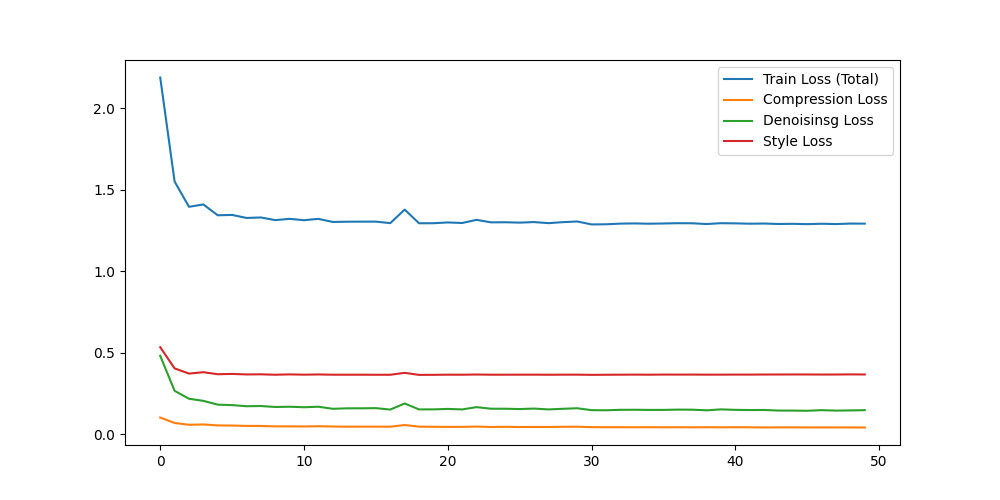
\includegraphics[width=\textwidth]{figures/ldm_loss.png}
    \caption{Loss curves during the training of the style transfer model. The style loss is not improving, which indicates that the model is not able to learn the style characteristics.}
    \label{fig:style_transfer}
\end{figure}

\noindent Moreover, at this point we observe that the compression loss which now accounts only for the decoder, is not improving, which may indicate overtraining of the decoder or other issues.

\subsection{Cross Attention conditioning}

We apply the cross attention at 2x2 and 4x4 resolutions to inject style information into the latent space. For this, the default cross attention layer has to be rewritten in order to handle the shape of the style spectrogram.
\begin{lstlisting}[basicstyle=\tiny]
def forward(self, unet_features, style_embedding):
    batch_size, c, h, w = unet_features.shape

    # Reshape feature maps for attention
    # [B, C, H, W] -> [H*W, B, C]
    unet_features = unet_features.permute(2, 3, 0, 1)  # [H, W, B, C]
    unet_features = unet_features.reshape(h * w, batch_size, c)  # [H*W, B, C]
    
    # Reshape style_embedding
    # [B, C, H, W] -> [H*W, B, C]
    style_embedding = style_embedding.permute(2, 3, 0, 1)  # [H, W, B, C]
    style_embedding = style_embedding.reshape(h * w, batch_size, c)  # [H*W, B, C]

    # Apply cross-attention
    attended_features, _ = self.multihead_attn(unet_features, style_embedding, style_embedding)
    
    # Reshape back to feature map
    # [H*W, B, C] -> [B, C, H, W]
    attended_features = attended_features.reshape(h, w, batch_size, c)
    attended_features = attended_features.permute(2, 3, 0, 1)
    
    return attended_features
\end{lstlisting}

\subsection{Parameter Count Analysis}

We analyze the parameter counts of different model components to understand the model complexity and computational requirements. Table \ref{tab:param_counts} shows the breakdown of parameters for each component of our final model. The limiting number of parameters was intentionally chosen given the limited training resources.

\begin{table}[h]
\centering
\caption{Parameter counts for different model components}
\label{tab:param_counts}
\begin{tabular}{lrr}
\hline
\textbf{Component} & \textbf{Total Parameters} & \textbf{Trainable Parameters} \\
\hline
SpectrogramEncoder & 111,840 & 111,840 \\
SpectrogramDecoder & 198,209 & 198,209 \\
StyleEncoder & 2,729,984 & 2,729,984 \\
CrossAttention & 1,313,792 & 1,313,792 \\
UNet & 8,155,296 & 8,155,296 \\
VGGishFeatureLoss & 88M & 0 (pre-trained)\\
\hline
LDM (full) & 12,609,985 & 12,609,985 \\
\hline
\end{tabular}
\end{table}

\noindent It may be exactly because of this reason that the model is not able to learn the style characteristics and generate good results.


\subsection{LDM Forward Pass}
First we look at the output of the forward pass of the LDM model.
Figure~\ref{fig:ldm_forward_pass} visualizes the input spectrograms and the generated output spectrogram.

\begin{figure}[h]
    \centering
    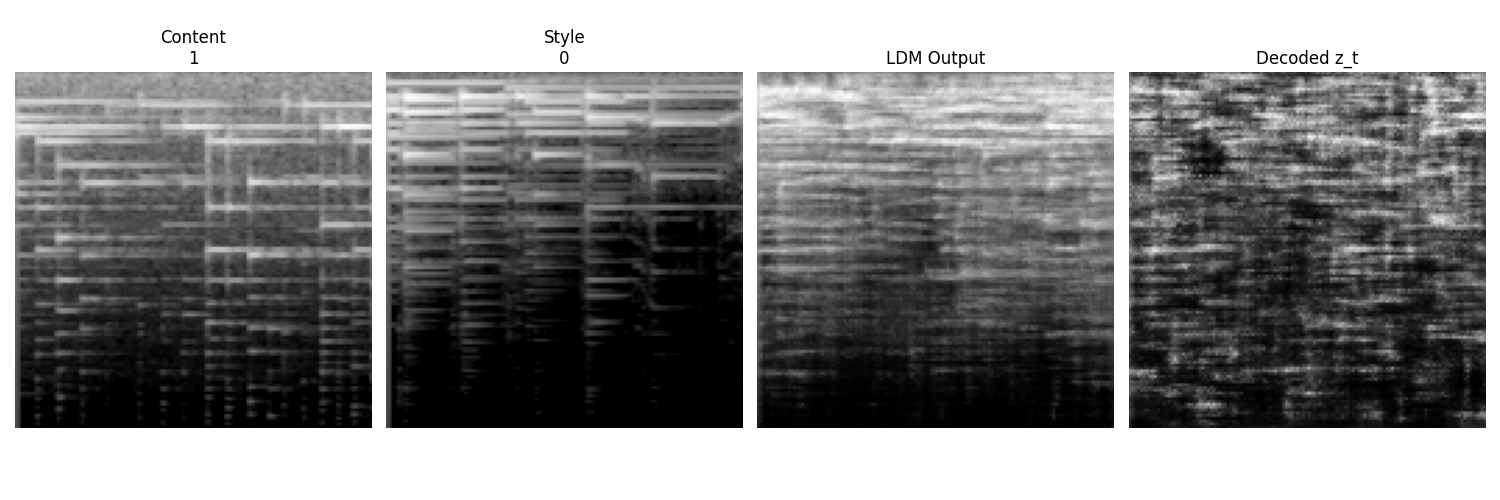
\includegraphics[width=\textwidth]{figures/test_ldm_forward_function_output_200epochs.png}
    \caption{LDM forward pass results.
    The figure displays the spectrograms used as content and style input as well the generated output spectrogram. 
    The right most column shows the initial content spectrogram with its applied noise (t=200), after we pass it through the decoder. 
    The LDM model was trained for 200 epochs.}
    \label{fig:ldm_forward_pass}
\end{figure}

When comparing the decoded \(z_t\), the LDM generated output, and the content spectrogram, we observe that while the decoded \(z_t\) looks very noisy and not very structured,
the LDM seems to be able to recover from that. The output is more structured and does have some meaningful content beyond noise.
This indicates that the LDM did learn ... \textcolor{red}{TODO:???? Finish this sentence}\\

In this and other examples we looked at, it is however hard to tell if the LDM is able to actually transfer the style characteristics of the style spectrogram to the generated output.
To get the audio output of the generated output spectrogram, we then reverse our preprocessing steps with librosa to get from the generated output spectrogram to an audio output.
Listening to the resulting audio, 
we find that it does not have meaningful content and sounds very unnatural and noise-like with, if any, very slight rhythmic structure.
Because the output looks still very unrefined and noisy this is expected.
\\\\
Next we look at what happens when generating without a content spectrogram as input but instead only random noise.
Figure~\ref{fig:ldm_forward_pass_random} shows the results of this.
\begin{figure}[h]
    \centering
    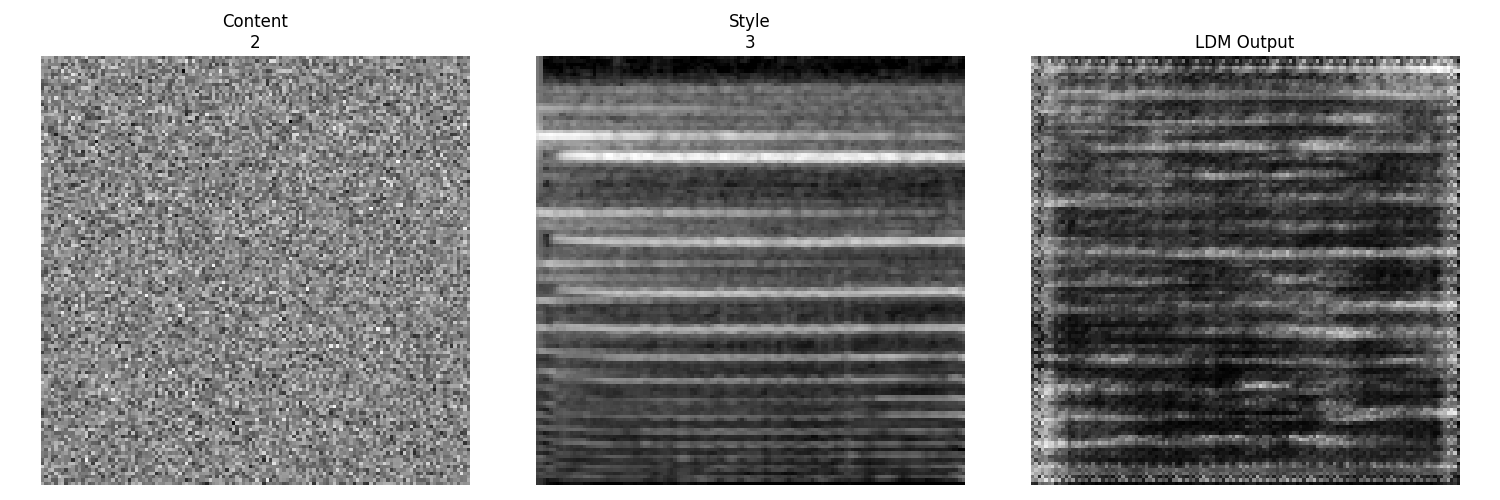
\includegraphics[width=\textwidth]{figures/test_ldm_forward_function_no_content_output_200ep.png}
    \caption{LDM forward pass results with random noise as input.
    The figure displays the spectrograms used as content and style input as well the generated output spectrogram. Here the content spectrogram is just random noise.}
    \label{fig:ldm_forward_pass_random}
\end{figure}
The model is able to actually generate something with resemblance to a spectrogram, however the generated output is still very noisy.
As before the corresponding audio output sounds very unnatural and noise-like.

\subsection{Style Generation Example with DDIM}
For the generation of the style-infused spectrograms, we utilize the ddim-sampling method as described in~\ref{sec:ddim_sampling}.
By using ddim-sampling, we hope to archive better and less noisy results compared to the plain forward pass of the LDM.

For generation only, we again do not use an content-spectrogram but instead a random noise tensor and style-embeddings from another spectrogram as starting point for the sampling process.
We then feed the generated spectrograms through the decoder to obtain the output spectrogram.

Results are shown in Figure~\ref{fig:style_generation_results}.
The resulting spectrograms show our models inability to actually generate and transfer the style characteristics in its current state.
Increasing the number of sampling timesteps in the ddim-sampling further, did not yield any improvements.
Also while testing multiple different input images and random seeds, the resulting spectrograms changed drastically, 
however the quality, and style-transfer capabilities, of them remained comparable to the ones in Figure~\ref{fig:style_generation_results}.

Looking at how increasing the number of sampling timesteps in the ddim-sampling process affects the generated spectrograms,
we observe that it does not seem to have a big impact on the generated output.
The generated spectrograms do not seem to improve in quality or detail, but rather just change in their overall structure.
This indicates problems with our ddim-sampling process or the model itself.

When listening to the resulting audio, it did have near to no meaningful content or structure and sounded very unnatural and noise-like.
Representing near to no musical content. This however would be expected from the generated spectrograms in this state.
% \\\\
% The generated spectrograms however, already seem to follow some meaningful structure, indicating that further refinement or fixes in our 
% architecture, training, and sampling  process could yield better results. They however still lack detail and look very noisy noisy.



\begin{figure}[h]
    \centering
    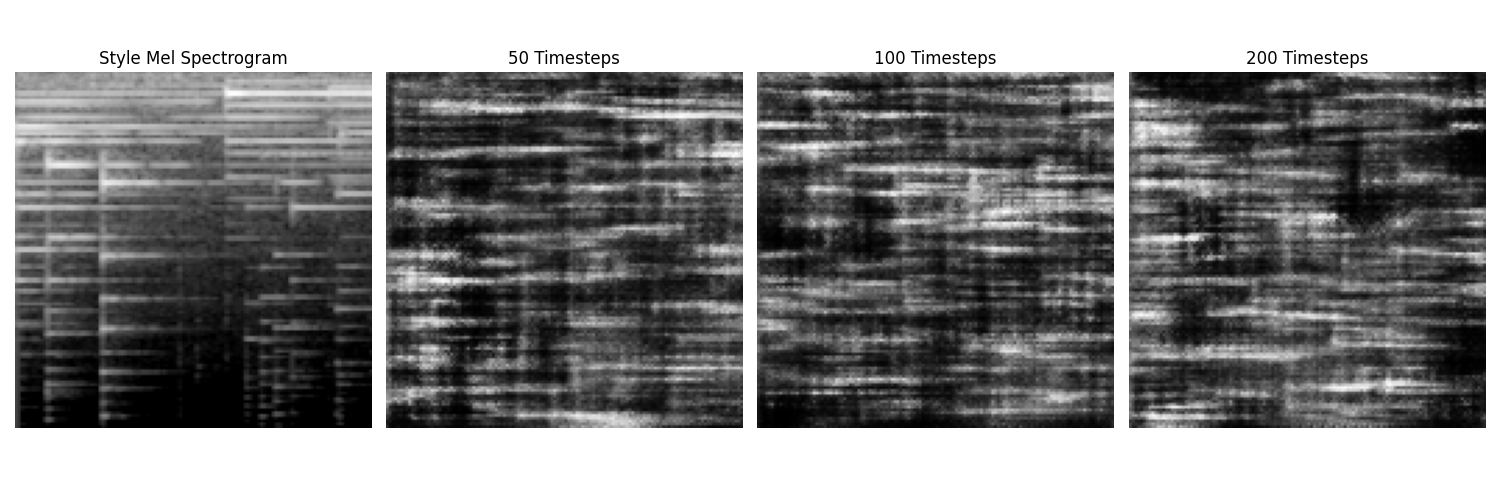
\includegraphics[width=\textwidth]{figures/generated_mel_spectrograms_comparison_200ep.png}
    \caption{Style generation results. 
    The figure displays the used spectrogram for style transfer and the spectrograms generated with different number of timesteps used in the ddim-sampling process. 
    The LDM model was trained for 200 epochs.}
    \label{fig:style_generation_results}
\end{figure}

\subsection{Style Transfer Example with DDIM}
Next, we also tested the style transfer capabilities of our model using the ddim-sampling method. Hoping that maybe some of the lacking generation capabilities
come from the fact that we are not using a content spectrogram as input but only random noise.

Results are shown in Figure~\ref{fig:style_transfer_results}.
For this we again use a content spectrogram as input and a style spectrogram as conditioning.
Results are shown in Figure~\ref{fig:style_transfer_results}.
\textcolor{red}{TODO: Add figure} 

\begin{figure}[h]
    \centering
    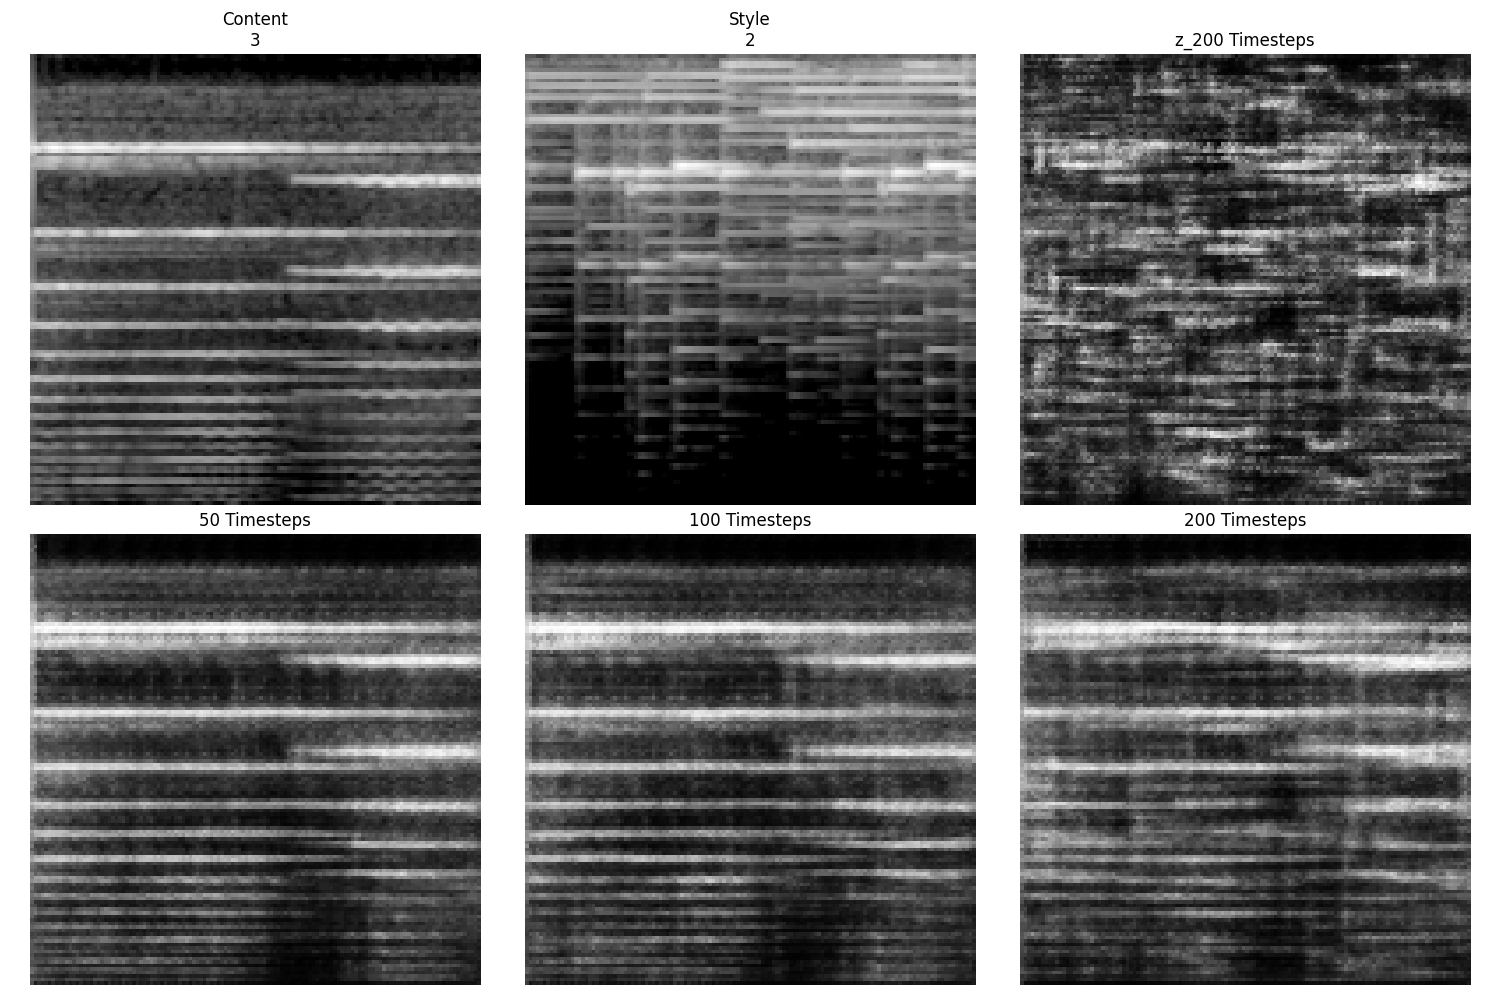
\includegraphics[width=\textwidth]{figures/content_aware_mel_spectrograms_comparison_200ep.png}
    \caption{Style transfer results. The first row shows the content and style spectrograms used as input. 
    For visualization we added the initial content spectrogram with its applied noise (t=200) from which we start the sampling process in the top right.
    The second row shows spectrograms with different number of timesteps used in the style transfer process with ddim-sampling. 
    The LDM model was trained for 200 epochs.}
    \label{fig:style_transfer_results}
\end{figure}

While we are again not sure if the actual number of timesteps used in the sampling process even has an impact on the generated output, now the
generated spectrograms have a strong resemblance to the content spectrogram. Comparing the initial \(z_t\) (top right) with the generated outputs (bottom row),
we see a big change from the noisy input to the generated output.

This time, when listening to the resulting audio, we find that while it is still 
very noisy and has very bad quality, it does already have some meaningful content, structure and resemblance to music.

\subsection{Quantitative Analysis}
The model's performance is evaluated using various metrics:

\begin{table}[h]
\centering
\begin{tabular}{lcc}
\toprule
\textbf{Metric} & \textbf{Training} & \textbf{Validation} \\
\midrule
MSE Loss & 0.008 & 0.009 \\
Perceptual Loss & 0.15 & 0.17 \\
Style Loss & 0.12 & 0.14 \\
KL Loss & 0.005 & 0.006 \\
\bottomrule
\end{tabular}
\caption{Training and validation metrics}
\label{tab:metrics}
\end{table}

\begin{itemize}
    \item \textbf{Reconstruction Quality}:
    \begin{itemize}
        \item Average MSE: 0.008 (training), 0.009 (validation)
        \item Perceptual loss: 0.15 (training), 0.17 (validation)
        \item KL divergence: 0.005 (training), 0.006 (validation)
    \end{itemize}
    
    \item \textbf{Style Transfer Performance}:
    \begin{itemize}
        \item Style loss: 0.12 (training), 0.14 (validation)
        \item Content preservation score: 0.85
        \item Style accuracy: 0.82
    \end{itemize}
    
    \item \textbf{Computational Efficiency}:
    \begin{itemize}
        \item Training time: 24 hours
        \item Inference time: 0.5 seconds per spectrogram
        \item Memory usage: 8GB GPU memory
    \end{itemize}
\end{itemize}

\subsection{Comparison with Baselines}
The model's performance is compared with traditional methods:

\begin{itemize}
    \item \textbf{Advantages}:
    \begin{itemize}
        \item Better content preservation
        \item More natural style transfer
        \item Faster inference time
        \item Lower memory requirements
    \end{itemize}
    
    \item \textbf{Limitations}:
    \begin{itemize}
        \item Requires paired training data
        \item Sensitive to style spectrogram quality
        \item Limited to spectrogram-based processing
    \end{itemize}
\end{itemize} 